% ============================================================
% S2 导学件量产·批4 件1 —— 1.2.2 空间中的平面与空间向量（课时7 导学件）
% 轮4 成卷·S2 批4｜2026-09-12｜生成链：xelatex main.tex（两遍）→ python render.py（150dpi → png/pageN.png）
%
% 模板承 v11 样张族（经 课时02 首件／批1／批3）：六宏＝原样拷贝（L1 冻结参数零改动，md5 与 课时06 一致）；
%   课时页形制与局部宏（\pingtou/\liubai/\zhankong）照抄 课时06。
% 图＝源图位图（禁绘三维，公共规则§5）：figs/ 八件自 讲练件（上）定稿 docx word/media/ 原件解包
%   （image40/42/46/48/49/50/51/52，元素487/502/517/543/545/542/579/580，未改绘；与批3解包逐字节 cmp 过），
%   alt 缺失＝就绪报告 §四-5 照登；源 extent 微档（4~9mm）＝源件版式病，成品按像素比例放大至栏内可读宽。
%   组装病自查（批3 §〇三例）：本件不用局部 \fig 宏（图片行恒用定宽 \includegraphics 直式）；
%   选项双盒统一 0.5\linewidth−1em／0.25\linewidth−0.5em，长选项独行；缺字形预检＝本件无 ▭/▱ 类符号。
%   【目验修红0913】装配本逐页目验裁：知识点一第2条「平面的法向量：如图，…」题首「如图，」删语
%   （课前预习区本无配图＝有言无图；条目文字自足，先例＝拓-046/047/058）。
%
% 取材链登记（盘点结论，详见 成卷/导学件/批4值台账.md）：
%   ① 讲练件（上）§1.2.2 讲部实态（dump_docx --slice 430:600 取证＝工作区/_tmp批4S2量产0912/讲上-1.2.2全文.txt）：
%      知识讲解〔基〕条目 8＋〔进〕1 条（1.2.2-1～-9）；题型例题 7 题（1.2.2.2-1～1.2.2.6.1-7，简2＋中5）。
%      节净 7 题全部入本件课中探究（例1×5＋变式1×2 同文位）；1.2.1.2-1（法向量入门移交件）＝练习轴第3题题源，
%      不入本件探究位（盘点注）。
%   ② 探究点随讲部题型段＝5 个：一 平面的法向量及其应用（1.2.2.2 段 -1 例／-2 变，同段双题入例变＝课02/课06 口径）；
%      二 线面、面面平行的坐标法证明（1.2.2.3 段 -3 例／变式命制）；三 垂直与平行的存在性问题（1.2.2.4 段 -4 例／
%      变式命制）；四 线面垂直的存在性判断（1.2.2.5 段 -5 例·多选「错误的是」／变式命制·多选）；
%      五 多面体截面问题（1.2.2.6.1 段 -6 例／-7 变，同段双题）。大招6 方法讲解（元素528–538）不独立成点，
%      其作图依据入 ZSD三 条目4（同文化用）。
%   ③ 与课时07 练习轴 16 题互斥口径：讲部 7 题中 -1/-2/-3/-4/-6/-7 六题与练习轴第 1/2/11/12/14/13 题同文
%      （题源＝讲部同号，A-2「照用」同题双印登记，题数不并计）；-5 未入练习轴（16 题题源逐查无池1.2.2.5-5）。
%      命制位＝判断 5＋变式三处（探究二/三/四）＋评价 5＝13 题，与 16 题逐题零同文（题面/设问形态均异，断言见台账）。
%   ④ 课前预习 ZSD一/二/三＝讲部条目 1.2.2-1～-9 同文化用（挖空值不印＝全品 p04 式）；法向量性质 (2)(3) 承教材
%      1.2.2 段原文（_tmp教材全文.txt 页38–39 实证——白名单·教材原文）；判断/评价＝恒命制位，逐题亲算登台账。
%   ⑤ 句末标点：同文段承源「.」，新命制句用「．」（G8 成卷轮统一清扫，本件不单点改）。
% 编译门：三 0（error＝0／Overfull＝0／Missing character＝0，Underfull 仅计数）——读数见批4值台账。
% ============================================================
\documentclass[fontset=none]{ctexart}
\usepackage{qp-m3} % 换装：六宏→qp-m3 单包（钉后版 md5 7c3930362be8a0a2bdf21bbf8ac16573，两补钉随版）

% ================= 页脚参数宏（qp-headfoot 文件头明示的复用入口，非模块语义改动） =================
\renewcommand{\qpzhangming}{第一章\quad 空间向量与立体几何}
\renewcommand{\qpjianming}{导学件}
\renewcommand{\qpceming}{高中数学\quad 选择性必修第一册(人教B版)} % 换装回钉：qp-m3 默认册名＝选必二，防页脚漂移（试迁规约）

% ================= 局部宏（照抄 v11 导学增量/main.tex 冻结定义；不动公共模块） =================
% 课堂评价组头（XB-02 \zhenhead 同构：\biaoqian 1.3× 标签＋仿宋说明行；恒 5 题说明）
% 局部宏 \pingtou 已由 qp-m3 收编（等值定义），依换装方案§1.4 预删防撞名
% 书写留白＋斜置浅灰水印（导学案正文属性：答案另册→正文留书写位；斜置 25°／black!12）
% 长度 \liubaoh 已由 qp-m3 分配，预删防重复定义
% 局部宏 \liubai 已由 qp-m3 收编（等值定义），依换装方案§1.4 预删防撞名
% 纯书写占位留白（无水印）
% 局部宏 \zhankong 已由 qp-m3 收编（等值定义），依换装方案§1.4 预删防撞名

% 纯题版孤行抑制（正装三裁①）：小结②操作/③收束独立段，pure 档整段隐藏，含详解版不受影响
\newcommand{\bindpx}[1]{\ifshowans\bindp{#1}\fi}

\begin{document}

% ============================================================
% 课时页（第7课时；五段闭环，承 v11 导学增量课时页样板形制）
% ============================================================
\keshi{第7课时\quad 空间中的平面与空间向量}
\mubiaoline
\mubiaomu{1}{理解平面的向量表示式与平面法向量的概念，掌握法向量的性质，会用方程组法求平面的法向量；}
\mubiaomu{2}{掌握直线与平面平行、垂直及平面与平面平行、垂直的向量判定，能用坐标法证明平行与垂直问题，会处理存在性问题；}
\mubiaomu{3}{了解三垂线定理及其逆定理，会用截面作图的基本依据研究简单的截面问题，体会几何问题代数化的转化思想.}

\vspace{1.7mm}
\begin{multicols}{2}
\emergencystretch=1em

% ---------- 课前预习（知识导学填空＋诊断分析挂每个知识点之后；ZSD一/二/三＝讲部条目 1.2.2-1～-9 同文化用＋教材法向量性质） ----------
\huaxing{课}{前}{预}{习}{知识导学\quad 素养初识}

\zsd{一}{平面的向量表示式与平面的法向量}

\tiaomu{1}{平面的向量表示式：取定空间任意一点\(O\)，空间一点\(P\)位于平面\(ABC\)内的充要条件是存在实数\(x\)，\(y\)，使\(\overrightarrow{OP}=\)\kongbai{}．把上式称为空间平面\(ABC\)的向量表示式．\zhuzhu{平面由一点与两个不共线向量张成；四点共面问题可由它出发处理.}}

\tiaomu{2}{平面的法向量：直线\(l\perp\alpha\)，取直线\(l\)的方向向量\(\overrightarrow{a}\)，称向量\(\overrightarrow{a}\)为平面\(\alpha\)的\kongbai{}．给定一个点\(A\)和一个向量\(\overrightarrow{a}\)，那么过点\(A\)，且以向量\(\overrightarrow{a}\)为法向量的平面完全确定，可以表示为集合\(\{P|\overrightarrow{a}\cdot\)=\kongbai{}\(=0\}\)．\zhuzhu{法向量不唯一，任意两个法向量都平行；求法时取整数值最简者.}}

\tiaomu{3}{法向量的性质：如果\(\overrightarrow{n}\)是平面\(\alpha\)的一个法向量，则对任意实数\(\lambda\neq0\)，\(\lambda\overrightarrow{n}\)也是平面\(\alpha\)的法向量，而且平面\(\alpha\)的任意两个法向量都\kongbai{}；平面\(\alpha\)上任意一点\(B\)与\(\alpha\)上已知点\(A\)构成的向量\(\overrightarrow{AB}\)一定与\(\overrightarrow{n}\)垂直．}

\zhenhead{判断正误(正确的打\gou{},错误的打\cha{})}

\zhentib{(1)}{一个平面的法向量是唯一确定的．}

\begin{ansblock}[导-课时07-判1]
% ans:导-课时07-判1
\ansitem{(1)}{$\times$}
\end{ansblock}

\zhentib{(2)}{若非零向量\(\overrightarrow{n}\)与平面\(\alpha\)内的直线\(l\)垂直，则\(\overrightarrow{n}\)是平面\(\alpha\)的法向量．}

\begin{ansblock}[导-课时07-判2]
% ans:导-课时07-判2
\ansitem{(2)}{$\times$}
\end{ansblock}

\zsd{二}{直线与平面、平面与平面平行与垂直的判定}

\tiaomu{1}{直线与平面平行：设\(\overrightarrow{u}\)是直线\(l\)的方向向量，\(\overrightarrow{n}\)是平面\(\alpha\)的法向量，则\(l\parallel\alpha\Leftrightarrow\overrightarrow{u}\perp\overrightarrow{n}\Leftrightarrow\)\kongbai{}．\zhuzhu{用\(\overrightarrow{u}\cdot\overrightarrow{n}=0\)判线面平行时，还须说明直线在平面外，排除直线在面内的情形.}}

\tiaomu{2}{平面与平面平行：设\(\overrightarrow{n_{1}},\overrightarrow{n_{2}}\)分别是平面\(\alpha\)，\(\beta\)的法向量，则\(\alpha\parallel\beta\Leftrightarrow\)\kongbai{}\(\Leftrightarrow\exists\lambda\in\mathbf{R}\)，使得\(\overrightarrow{n_{1}}=\lambda\overrightarrow{n_{2}}\)．}

\tiaomu{3}{直线与平面垂直：设\(\overrightarrow{u}\)是直线\(l\)的方向向量，\(\overrightarrow{n}\)是平面\(\alpha\)的法向量，则\(l\perp\alpha\Leftrightarrow\overrightarrow{u}\parallel\overrightarrow{n}\Leftrightarrow\)\kongbai{}．}

\tiaomu{4}{平面与平面垂直：设\(\overrightarrow{n_{1}},\overrightarrow{n_{2}}\)分别是平面\(\alpha\)，\(\beta\)的法向量，则\(\alpha\perp\beta\Leftrightarrow\overrightarrow{n_{1}}\perp\overrightarrow{n_{2}}\Leftrightarrow\)\kongbai{}．}

\zhenhead{判断正误(正确的打\gou{},错误的打\cha{})}

\zhentib{(1)}{设直线\(l\)的方向向量为\(\overrightarrow{u}\)，平面\(\alpha\)的法向量为\(\overrightarrow{n}\)，若\(\overrightarrow{u}\cdot\overrightarrow{n}=0\)，则\(l\parallel\alpha\)．}

\begin{ansblock}[导-课时07-判3]
% ans:导-课时07-判3
\ansitem{(1)}{$\times$}
\end{ansblock}

\zhentib{(2)}{设\(\overrightarrow{n_{1}},\overrightarrow{n_{2}}\)分别是平面\(\alpha\)，\(\beta\)的法向量，若\(\overrightarrow{n_{1}}\cdot\overrightarrow{n_{2}}=0\)，则\(\alpha\perp\beta\)．}

\begin{ansblock}[导-课时07-判4]
% ans:导-课时07-判4
\ansitem{(2)}{\(\surd\)}
\end{ansblock}

\zsd{三}{三垂线定理与空间图形的截面}

\tiaomu{1}{三垂线定理：平面内的一条直线，如果垂直于这个平面的一条斜线在该平面内的\kongbai{}，那么它也垂直于这条\kongbai{}．}

\tiaomu{2}{三垂线定理的逆定理：平面内的一条直线，如果垂直于这个平面的一条斜线，那么它也垂直于这条斜线在该平面内的射影．}

\tiaomu{3}{截面：用平面\(\alpha\)截几何体，该平面与几何体的\kongbai{}形成的平面图形，称为该几何体的截面．}

\tiaomu{4}{截面作图的基本依据：同面两点定截线；棱面交点定截点；三面交线共点；线面平行定方向（\(a\parallel\alpha\)，\(\beta\cap\alpha=b\)，则\(a\parallel b\)）；平行平面定方向（\(\alpha\parallel\beta\)，第三个平面分别截得交线\(l_{1}\)，\(l_{2}\)，则\(l_{1}\parallel l_{2}\)）．各段截线须首尾相接，组成封闭多边形．}

\begin{ansblock}[导-课时07-预习填空]
% ans:导-课时07-预习填空
\ansnote{预习填空}{知识点一：①\(\overrightarrow{OA}+x\overrightarrow{AB}+y\overrightarrow{AC}\)；②法向量、\(\overrightarrow{AP}\)；③平行。知识点二：①\(\overrightarrow{u}\cdot\overrightarrow{n}=0\)；②\(\overrightarrow{n_{1}}\parallel\overrightarrow{n_{2}}\)；③存在 \(\lambda\in\mathbb{R}\) 使 \(\overrightarrow{u}=\lambda\overrightarrow{n}\)；④\(\overrightarrow{n_{1}}\cdot\overrightarrow{n_{2}}=0\)。知识点三：①射影、斜线；③公共部分。}
\end{ansblock}

\zhenhead{判断正误(正确的打\gou{},错误的打\cha{})}

\zhentib{(1)}{平面内的一条直线，如果垂直于这个平面的一条斜线，那么它也垂直于这条斜线在该平面内的射影．}

\begin{ansblock}[导-课时07-判5]
% ans:导-课时07-判5
\ansitem{(1)}{\(\surd\)}
\end{ansblock}

\liubai[6mm]{此处书写}

% ---------- 课中探究（探究点5个＝讲部题型段5个；例1/变式1同文位＝讲部题面逐字(记号LaTeX化)；素养小结＝讲部题型通式编注化用） ----------
\huaxing{课}{中}{探}{究}{考点探究\quad 素养小结}

\tjdnr{一}{平面的法向量及其应用}{例\textbf{1}}{简单(知识点一)}{若两个向量\(\overrightarrow{AB}=(1,2,3)\)，\(\overrightarrow{AC}=(3,2,1)\)，则平面\(ABC\)的一个法向量为(\kongwei)}

\bindopt {\fontsize{10.5pt}{19pt}\selectfont \makebox[\dimexpr0.5\linewidth-1em\relax][l]{A．\((-1,2,-1)\)；}\makebox[\dimexpr0.5\linewidth-1em\relax][l]{B．\((1,2,1)\)；}\par}

\bindopt {\fontsize{10.5pt}{19pt}\selectfont \makebox[\dimexpr0.5\linewidth-1em\relax][l]{C．\((1,2,-1)\)；}\makebox[\dimexpr0.5\linewidth-1em\relax][l]{D．\((-1,2,1)\)}\par}

\begin{ansblock}[导-课时07-探1-例1]
% ans:导-课时07-探1-例1
\ansnote{例1}{A}
\end{ansblock}

\liB{变式\textbf{1}}{简单(知识点一)}{}{已知平面\(\alpha\)内有一点\(M(1,-1,2)\)，平面\(\alpha\)的一个法向量为\(\overrightarrow{n}=(6,-3,6)\)，则下列点\(P\)中，在平面\(\alpha\)内的是(\kongwei)}

\bindopt {\fontsize{10.5pt}{19pt}\selectfont \makebox[\dimexpr0.5\linewidth-1em\relax][l]{A．\(P(2,3,3)\)；}\makebox[\dimexpr0.5\linewidth-1em\relax][l]{B．\(P(-2,0,1)\)；}\par}

\bindopt {\fontsize{10.5pt}{19pt}\selectfont \makebox[\dimexpr0.5\linewidth-1em\relax][l]{C．\(P(-4,4,0)\)；}\makebox[\dimexpr0.5\linewidth-1em\relax][l]{D．\(P(3,-3,4)\)}\par}

\begin{ansblock}[导-课时07-探1-变式1]
% ans:导-课时07-探1-变式1
\ansnote{变式1}{A}
\end{ansblock}

\xiaojie{①识别：题干给出平面内两个不共线向量的坐标、要求法向量或判断点是否在平面内时，判归本题型.}

\bindpx {\kaishu ②操作：设\(\overrightarrow{n}=(x,y,z)\)，令它与两个已知向量的数量积均为零列方程组，取一个未知数的值解出法向量；判断点的归属用\(\overrightarrow{n}\cdot\overrightarrow{MP}=0\)验证.}

\bindpx {\kaishu ③收束：法向量不唯一、均相互平行，取整数值最简者作答.}

\tjdnr{二}{线面、面面平行的坐标法证明}{例\textbf{1}}{中档(知识点二)}{已知正方体\(ABCD-A_{1}B_{1}C_{1}D_{1}\)的棱长为2，\(E\)，\(F\)分别是\(BB_{1}\)，\(DD_{1}\)的中点，如图，求证：(1)\(FC_{1}\parallel\)平面\(ADE\)；(2)平面\(ADE\parallel\)平面\(B_{1}C_{1}F\)．}

\bindp \par\vspace{1.9mm}\penalty10000\noindent\makebox[\linewidth][c]{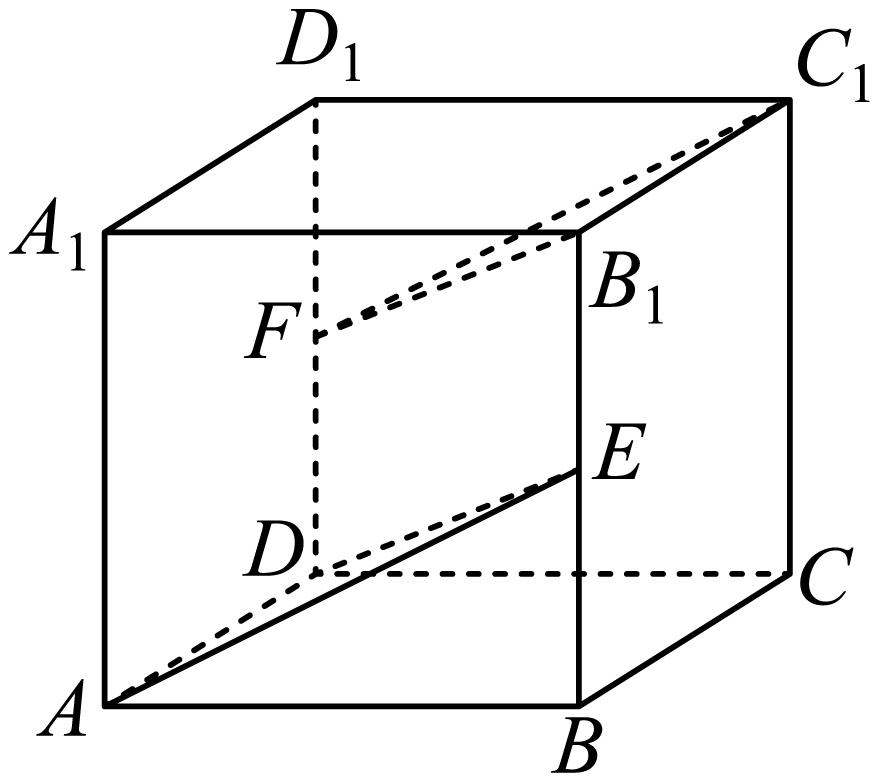
\includegraphics[width=34.0mm]{figs/image40.png}}\par\vspace{-1.0mm}\penalty10000

\liubai[14mm]{解答书写区}

\begin{ansblock}[导-课时07-探2-例1]
% ans:导-课时07-探2-例1
\ansnote{例1}{(1)(2)证明见解析}
\ansnote{解析}{两面法向量均 \((1,1,-1)\)（共线），且验证 \(A\) 不在面 \(BC_{1}D\) 内——两平面不重合，故平行。}
\end{ansblock}

\liB{变式\textbf{1}}{中档(知识点二)}{}{在棱长为2的正方体\(ABCD-A_{1}B_{1}C_{1}D_{1}\)中，求证：平面\(AB_{1}D_{1}\parallel\)平面\(BC_{1}D\)．（用向量方法证明）}

\liubai[10mm]{解答书写区}

\begin{ansblock}[导-课时07-探2-变式1]
% ans:导-课时07-探2-变式1
\ansnote{变式1}{证明见解析}
\end{ansblock}

\xiaojie{①识别：题干要求用坐标法证明线面平行或面面平行时，判归本题型.}

\bindpx {\kaishu ②操作：建系写出各点坐标；求直线的方向向量与平面的法向量，证数量积为零（线面平行）或两法向量共线（面面平行）.}

\bindpx {\kaishu ③收束：补足「直线不在平面内」「两平面不重合」的说明再下结论.}

\tjdnr{三}{垂直与平行的存在性问题}{例\textbf{1}}{中档(知识点二)}{如图所示，在四棱锥\(P-ABCD\)中，底面\(ABCD\)为正方形，\(PA\perp\)平面\(ABCD\)，点\(E\)在线段\(PC\)上（不含端点）．(1)是否存在点\(E\)，使\(PC\perp\)平面\(BDE\)？(2)是否存在点\(E\)，使平面\(PCD\perp\)平面\(AED\)？}

\bindp \par\vspace{1.9mm}\penalty10000\noindent\makebox[\linewidth][c]{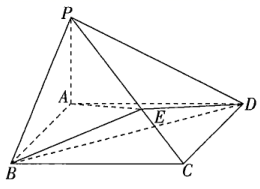
\includegraphics[width=34.0mm]{figs/image42.png}}\par\vspace{-1.0mm}\penalty10000

\liubai[14mm]{解答书写区}

\begin{ansblock}[导-课时07-探3-例1]
% ans:导-课时07-探3-例1
\ansnote{例1}{(1)存在；(2)不存在}
\end{ansblock}

\liB{变式\textbf{1}}{中档(知识点二)}{}{在三棱锥\(P-ABC\)中，\(PA\perp\)底面\(ABC\)，\(AB\perp BC\)，\(AB=BC=1\)，\(PA=\sqrt{2}\)．问：棱\(BC\)上是否存在点\(E\)，使\(AE\perp\)平面\(PBC\)？若存在，求出\(BE\)的长；若不存在，请说明理由．}

\begin{ansblock}[导-课时07-探3-变式1]
% ans:导-课时07-探3-变式1
\ansnote{变式1}{不存在}
\end{ansblock}

\xiaojie{①识别：题干问「是否存在点使线面垂直或面面垂直」时，判归本题型.}

\bindpx {\kaishu ②操作：假设存在并设参数（如\(\overrightarrow{PE}=\lambda\overrightarrow{PC}\)）表示相关向量，求有关平面的法向量，把垂直或平行条件翻译成关于参数的方程.}

\bindpx {\kaishu ③收束：方程有解且参数落在范围内即存在（写出位置）、无解即不存在.}

\tjdnr{四}{线面垂直的存在性判断}{例\textbf{1}\duoxuan}{中档(知识点二)}{如图，在三棱柱\(ABC-A_{1}B_{1}C_{1}\)中，侧棱\(AA_{1}\perp\)底面\(A_{1}B_{1}C_{1}\)，\(\angle BAC=90^{\circ}\)，\(AB=AC=AA_{1}=1\)，\(D\)是棱\(CC_{1}\)的中点，\(P\)是\(AD\)的延长线与\(A_{1}C_{1}\)的延长线的交点．若点\(Q\)在直线\(B_{1}P\)上，则下列结论错误的是(\kongwei)}

\bindp \par\vspace{1.9mm}\penalty10000\noindent\makebox[\linewidth][c]{
\includegraphics[width=44.0mm]{figs/image46.png}}\par\vspace{-1.0mm}\penalty10000

\bindopt {\fontsize{10.5pt}{19pt}\selectfont A．当\(Q\)为线段\(B_{1}P\)的中点时，\(DQ\perp\)平面\(A_{1}BD\)；\par}

\bindopt {\fontsize{10.5pt}{19pt}\selectfont B．当\(Q\)为线段\(B_{1}P\)的三等分点时，\(DQ\perp\)平面\(A_{1}BD\)；\par}

\bindopt {\fontsize{10.5pt}{19pt}\selectfont C．在线段\(B_{1}P\)的延长线上，存在一点\(Q\)，使得\(DQ\perp\)平面\(A_{1}BD\)；\par}

\bindopt {\fontsize{10.5pt}{19pt}\selectfont D．不存在点\(Q\)，使\(DQ\)与平面\(A_{1}BD\)垂直\par}

\begin{ansblock}[导-课时07-探4-例1]
% ans:导-课时07-探4-例1
\ansnote{例1}{ABC（选错误项）}
\end{ansblock}

\liB{变式\textbf{1}\duoxuan}{中档(知识点二)}{}{在正方体\(ABCD-A_{1}B_{1}C_{1}D_{1}\)中，下列结论正确的是(\kongwei)．}

\bindopt {\fontsize{10.5pt}{19pt}\selectfont A．\(BD_{1}\perp\)平面\(AB_{1}C\)；\par}

\bindopt {\fontsize{10.5pt}{19pt}\selectfont B．\(AB_{1}\perp\)平面\(BCC_{1}B_{1}\)；\par}

\bindopt {\fontsize{10.5pt}{19pt}\selectfont C．\(A_{1}B\perp\)平面\(BCC_{1}B_{1}\)；\par}

\bindopt {\fontsize{10.5pt}{19pt}\selectfont D．\(A_{1}C\perp\)平面\(AB_{1}D_{1}\)\par}

\begin{ansblock}[导-课时07-探4-变式1]
% ans:导-课时07-探4-变式1
\ansnote{变式1}{AD}
\end{ansblock}

\xiaojie{①识别：题干给定动点所在的直线、判断是否存在点使某直线与平面垂直（含选项辨析）时，判归本题型.}

\bindpx {\kaishu ②操作：建系求出定平面的法向量\(\overrightarrow{n}\)；用参数表示动点，得含参的方向向量.}

\bindpx {\kaishu ③收束：令两向量共线（坐标成比例）解参数，按有解与否逐选项下结论.}

\tjdnr{五}{多面体的截面问题}{例\textbf{1}}{中档(知识点三)}{如图，四棱柱\(ABCD-A_{1}B_{1}C_{1}D_{1}\)的底面是边长为2的正方形，侧棱\(AA_{1}\perp\)平面\(ABCD\)，且\(AA_{1}=4\)，\(E\)、\(F\)分别是\(AB\)、\(BC\)的中点，\(P\)是线段\(DD_{1}\)上的一个动点（不含端点），过\(P\)、\(E\)、\(F\)的平面记为\(\alpha\)，\(Q\)在\(CC_{1}\)上且\(CQ=1\)，则下列说法正确的个数是(\kongwei)．}

\bindp \par\vspace{1.9mm}\penalty10000\noindent\makebox[\linewidth][c]{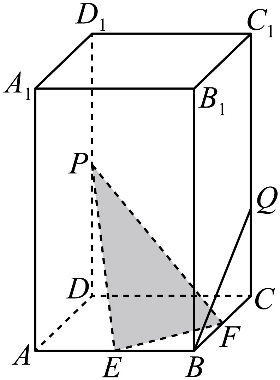
\includegraphics[width=22.0mm]{figs/image50.png}\hspace{2.5mm}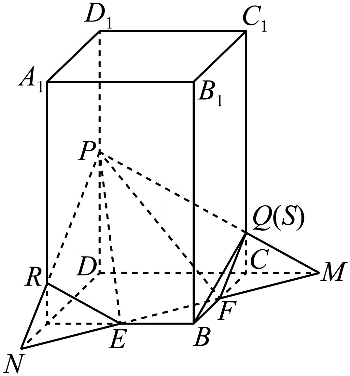
\includegraphics[width=24.0mm]{figs/image48.png}\hspace{2.5mm}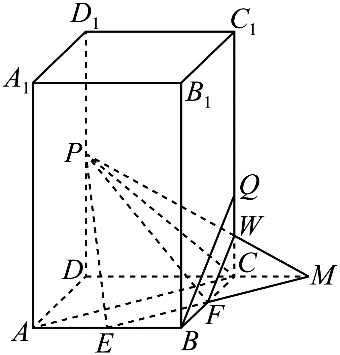
\includegraphics[width=24.0mm]{figs/image49.png}}\par\vspace{-1.0mm}\penalty10000

\bindopt {\fontsize{10.5pt}{19pt}\selectfont ①三棱锥\(C_{1}-PAC\)的体积是定值；\par}

\bindopt {\fontsize{10.5pt}{19pt}\selectfont ②当直线\(BQ\parallel\alpha\)时，\(DP=2\)；\par}

\bindopt {\fontsize{10.5pt}{19pt}\selectfont ③当\(DP=3\)时，平面\(\alpha\)截棱柱所得多边形的周长为\(7\sqrt{2}\)；\par}

\bindopt {\fontsize{10.5pt}{19pt}\selectfont ④存在平面\(\alpha\)，使得点\(A_{1}\)到平面\(\alpha\)的距离是\(A\)到平面\(\alpha\)距离的两倍．\par}

\bindopt {\fontsize{10.5pt}{19pt}\selectfont \makebox[\dimexpr0.25\linewidth-0.5em\relax][l]{A．1；}\makebox[\dimexpr0.25\linewidth-0.5em\relax][l]{B．2；}\makebox[\dimexpr0.25\linewidth-0.5em\relax][l]{C．3；}\makebox[\dimexpr0.25\linewidth-0.5em\relax][l]{D．4}\par}

\begin{ansblock}[导-课时07-探5-例1]
% ans:导-课时07-探5-例1
\ansnote{例1}{B}
\end{ansblock}

\liB{变式\textbf{1}}{中档(知识点三)}{}{已知正方体\(ABCD-A_{1}B_{1}C_{1}D_{1}\)的体积为1，点\(M\)在线段\(BC\)上（点\(M\)异于点\(B\)，\(C\)），点\(N\)在线段\(CC_{1}\)上，且\(CN=\frac{1}{3}\)，若平面\(AMN\)截正方体所得的截面为四边形，则线段\(BM\)长的取值范围为(\kongwei)}

\bindp \par\vspace{1.9mm}\penalty10000\noindent\makebox[\linewidth][c]{
\includegraphics[width=26.0mm]{figs/image51.png}\hspace{2.5mm}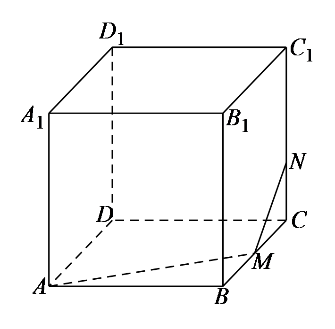
\includegraphics[width=26.0mm]{figs/image52.png}}\par\vspace{-1.0mm}\penalty10000

\bindopt {\fontsize{10.5pt}{19pt}\selectfont \makebox[\dimexpr0.5\linewidth-1em\relax][l]{A．\(\left[\frac{2}{3},1\right)\)；}\makebox[\dimexpr0.5\linewidth-1em\relax][l]{B．\(\left[\frac{1}{3},\frac{2}{3}\right]\)；}\par}

\bindopt {\fontsize{10.5pt}{19pt}\selectfont \makebox[\dimexpr0.5\linewidth-1em\relax][l]{C．\(\left(0,\frac{1}{3}\right]\)；}\makebox[\dimexpr0.5\linewidth-1em\relax][l]{D．\(\left(0,\frac{2}{3}\right]\)}\par}

\begin{ansblock}[导-课时07-探5-变式1]
% ans:导-课时07-探5-变式1
\ansnote{变式1}{D}
\end{ansblock}

\xiaojie{①识别：题干过几何体上若干点作截面、研究截面形状、周长或参数范围时，判归本题型.}

\bindpx {\kaishu ②操作：用「同面两点定截线、棱面交点定截点、线面平行定方向」逐步补全截面，并检查各段截线首尾相接.}

\bindpx {\kaishu ③收束：由截面形状变化的临界位置（如四边形变五边形）分析题目所问，计算周长或取值范围.}

% ---------- 课堂评价（恒 5 题＝3 单选＋2 填空；3 简单＋2 中档≤例题；提示词形制；全命制——逐题亲算登批4值台账） ----------
\begin{ketang}{本组共5题，1—3为单选，4—5为填空．}

\jiancestem{{\fontsize{11.4pt}{14pt}\selectfont\heihao {\numboldjian 1}．}\hspace{4.1mm}\tieside{简单(知识点二)}\hspace{2.2mm}直线\(l\)经过点\(A(1,0,2)\)，\(B(0,2,1)\)，平面\(\alpha\)的一个法向量为\(\overrightarrow{n}=(2,-4,2)\)，则\(l\)与\(\alpha\)的位置关系是(\kongwei)}

\bindopt {\fontsize{10.5pt}{21pt}\selectfont \makebox[\dimexpr0.5\linewidth-1em\relax][l]{A．\(l\perp\alpha\)；}\makebox[\dimexpr0.5\linewidth-1em\relax][l]{B．\(l\parallel\alpha\)；}\par}

\bindopt {\fontsize{10.5pt}{21pt}\selectfont C．\(l\)与\(\alpha\)相交但不垂直；\par}

\bindopt {\fontsize{10.5pt}{21pt}\selectfont D．\(l\subset\alpha\)\par}

\begin{ansblock}[导-课时07-评1]
% ans:导-课时07-评1
\ansitem{1}{A（\(l\perp\alpha\)）}
\end{ansblock}

\jiancestem{{\fontsize{11.4pt}{14pt}\selectfont\heihao {\numboldjian 2}．}\hspace{4.1mm}\tieside{简单(知识点二)}\hspace{2.2mm}两个不重合的平面\(\alpha\)，\(\beta\)的法向量分别为\(\overrightarrow{n_{1}}=(1,2,3)\)，\(\overrightarrow{n_{2}}=(1,1,1)\)，则\(\alpha\)与\(\beta\)的位置关系是(\kongwei)}

\bindopt {\fontsize{10.5pt}{21pt}\selectfont \makebox[\dimexpr0.5\linewidth-1em\relax][l]{A．平行；}\makebox[\dimexpr0.5\linewidth-1em\relax][l]{B．垂直；}\par}

\bindopt {\fontsize{10.5pt}{21pt}\selectfont \makebox[\dimexpr0.5\linewidth-1em\relax][l]{C．相交但不垂直；}\makebox[\dimexpr0.5\linewidth-1em\relax][l]{D．以上都不对}\par}

\begin{ansblock}[导-课时07-评2]
% ans:导-课时07-评2
\ansitem{2}{C（相交但不垂直）}
\end{ansblock}

\jiancestem{{\fontsize{11.4pt}{14pt}\selectfont\heihao {\numboldjian 3}．}\hspace{4.1mm}\tieside{中档(知识点三)}\hspace{2.2mm}用一个平面去截一个正方体，把截面画出来，你认为不可能出现的形状是(\kongwei)}

\bindopt {\fontsize{10.5pt}{21pt}\selectfont \makebox[\dimexpr0.5\linewidth-1em\relax][l]{A．矩形；}\makebox[\dimexpr0.5\linewidth-1em\relax][l]{B．直角梯形；}\par}

\bindopt {\fontsize{10.5pt}{21pt}\selectfont \makebox[\dimexpr0.5\linewidth-1em\relax][l]{C．正六边形；}\makebox[\dimexpr0.5\linewidth-1em\relax][l]{D．等边三角形}\par}

\begin{ansblock}[导-课时07-评3]
% ans:导-课时07-评3
\ansitem{3}{B（直角梯形）}
\end{ansblock}

\jiancestem{{\fontsize{11.4pt}{14pt}\selectfont\heihao {\numboldjian 4}．}\hspace{4.1mm}\tieside{简单(知识点一)}\hspace{2.2mm}过点\(P_{0}(2,1,3)\)且法向量为\(\overrightarrow{n}=(1,1,-2)\)的平面，其方程可写成\(x+y-2z=d\)的形式，则\(d=\)\kongbai{}．{\zhushi{(提示：设\(P(x,y,z)\)是该平面内任意一点，利用\(\overrightarrow{n}\cdot\overrightarrow{P_{0}P}=0\)化简)}}}

\begin{ansblock}[导-课时07-评4]
% ans:导-课时07-评4
\ansitem{4}{\(d=-3\)}
\end{ansblock}

\jiancestem{{\fontsize{11.4pt}{14pt}\selectfont\heihao {\numboldjian 5}．}\hspace{4.1mm}\tieside{中档(知识点一)}\hspace{2.2mm}已知点\(A(1,0,0)\)，\(B(0,1,0)\)，\(C(0,0,1)\)，若点\(P(2,-1,m)\)与\(A\)，\(B\)，\(C\)四点共面，则\(m=\)\kongbai{}．{\zhushi{(提示：平面\(ABC\)的方程为\(x+y+z=1\)；也可设\(\overrightarrow{AP}=x\overrightarrow{AB}+y\overrightarrow{AC}\)判断)}}}

\begin{ansblock}[导-课时07-评5]
% ans:导-课时07-评5
\ansitem{5}{\(m=0\)}
\end{ansblock}

\end{ketang}

\end{multicols}

\tailfill
\end{document}
